%%%%%%%%%%%%%%%%%%%%%%%%%%%%%%%%%%%%%%%%%
% Medium Length Professional CV
% LaTeX Template
% Version 2.0 (8/5/13)
%
% This template has been downloaded from:
% http://www.LaTeXTemplates.com
%
% Original author:
% Trey Hunner (http://www.treyhunner.com/)
%
% Important note:
% This template requires the resume.cls file to be in the same directory as the
% .tex file. The resume.cls file provides the resume style used for structuring the
% document.
%
%%%%%%%%%%%%%%%%%%%%%%%%%%%%%%%%%%%%%%%%%

%----------------------------------------------------------------------------------------
% PACKAGES AND OTHER DOCUMENT CONFIGURATIONS
%----------------------------------------------------------------------------------------

\documentclass{resume} % Use the custom resume.cls style

\usepackage[left=0.75in,top=0.3in,right=0.75in,bottom=0.3in]{geometry} % Document margins
\usepackage{verbatim}
\usepackage[colorlinks,urlcolor=blue]{hyperref}
\usepackage{tabularx}
\usepackage{graphicx}
\graphicspath{ {./images/} }

\name{Alexander Myltsev}
\address{
  email: \href{mailto:alexander@myltsev.com}{alex@myltsev.com} $\vert$
  skype: alexander.myltsev $\vert$
  github: \href{https://github.com/alexander-myltsev/}{alexander-myltsev}
}
\address{CV update: April, 2019 $\vert$ \href{http://myltsev.com/cv}{http://myltsev.com/cv}}

\begin{document}

%----------------------------------------------------------------------------------------
% EDUCATION SECTION
%----------------------------------------------------------------------------------------

\begin{rSection}{Education}

%------------------------------------------------

\begin{rSubsectionEducation}{Moscow Institute of Physics and Technology}{MIPT}{Moscow,
Russia, 2008--2010}{Department of Control and Applied Mathematics, 
subdepartment of Informatics (CIS)}
\item \textit{M.Sc. in Mathematics and Computer Science}, GPA: 5.0/5.0
\item \textit{Thesis:} Embedding Domain Specific Language in F\# for Hybrid System Control
\item \textit{Advisor:} \href{https://ru.linkedin.com/in/andreyustyuzhanin}{Andrey Ustyuzhanin},
Ph.D. in CS, Associate Professor at MIPT, Head of joint CERN-Yandex Research \& Education programs
\end{rSubsectionEducation}

%------------------------------------------------

\begin{rSubsectionSchools}{Self Education, Coursera}
\item \href{https://yandexdataschool.com/}{Yandex School of Data Analysis} (completed 2 of 4 semesters)
\item \href{https://www.coursera.org/specializations/machine-learning-data-analysis}
{``Machine Learning Data Analysis'' specialization by MIPT and Yandex}, Coursera (completed 5 of 6 courses, 100\% grade, currently working on the final project)
\item ``Competitive Data Science`` by \href{https://www.facebook.com/groups/data.mining.in.action/}{AppliedDataScience}.
Lecturers and tutors from Higher School of Economics, Moscow Institute of Physics and Technology,
Yandex. Certified, \href{https://docs.google.com/spreadsheets/d/1jFqmeIUA7gnFFApWf7_YrefQ2XT8TcSl2M_t68gpIOY/edit#gid=511559587}{rating: 7th out of 116 students}
\item ``Algorithms: Design and Analysis'' by Tim Roughgarden, Stanford University. 70\% grade
\item ``Machine Learning'' by Andrew Ng, Stanford University. 100\% grade
\item ``Principles of Reactive Programming in Scala'' by Martin Odersky et al., EPFL. 98.2\% grade
\item ``Functional Programming Principles in Scala'' by Martin Odersky et al., EPFL. 100\% grade
\item ``Structure and Interpretation of Computer Programs'' by H. Abelson and G. J. Sussman.
Solely solved all exercises of the book
\item ``Personal Assets Allocation Management'' specialization by
      \href{https://finarium.pro/}{Finarium.pro}. 90\% grade
\end{rSubsectionSchools}
\end{rSection}

%----------------------------------------------------------------------------------------
% ACADEMIC CONTRIBUTIONS SECTION
%----------------------------------------------------------------------------------------

\begin{rSubsectionSchools}{Academic Contributions}
\item Paper ``parboiled2: macro-based parsing expression grammar generator for Scala programming
language''. Journal of Functional Programming (ISSN: 1469-7653, Online)
\textit{(\href{http://myltsev.com/papers/parboiled2.pdf}{draft})}
\item Paper \href{https://bmcbioinformatics.biomedcentral.com/articles/10.1186/s12859-017-1663-3}
{``gnparser'': a powerful parser for scientific names based on Parsing Expression Grammar''}.
BioMed Central (Software) journal (DOI: 10.1186/s12859-017-1663-3)
\item Manning Press books reviewer. Books include:
``Type-Driven Development with Idris'' by Edwin Brady,
``Practical Recommender Systems'' by Kim Falk,
``Machine Learning with TensorFlow'' by Nishant Shukla,
``Deep Learning with Python'' by Francois Chollet,
``The Tao of Microservices'' by Richard Rodger,
``Kubernetes in Action'' by Marko Lukša,
``Grokking Deep Learning'' by Andrew W. Trask
\item Co-author of the book ``Parallel computing on GPU Architecture and CUDA programming  model''
\item Mozilla Labs article:
\href{http://myltsev.com/2015/Elevating-JavaScript-Performance-Through-GPU-Power/}{``Elevating
 JavaScript Performance Through GPU Power''}
\end{rSubsectionSchools}

%------------------------------------------------

\begin{rSubsectionSchools}{Summer/Winter Schools}
\item July '15, participant of \href{http://game.deephack.me/}{``Deephack.Game''
(http://game.deephack.me)} -- deep neural
networks week conference and hackathon at \href{http://mipt.ru/}{Moscow Institute of Physics and
Technology}
% \item Oct '13, Participant of ``Start in Garage'' two days startup acceleration program at
% MIPT. Organized by \href{http://www.risventures.com/}{RIS Ventures}
\item Aug '14, 8th Russian Summer School in Information Retrieval (RuSSIR)
\item July '11, Summer School in Software Engineering and Verification. Best project award for
``Formally Proving Facts in the Refinement Algebra'' Mentor: Sir Tony Hoare, Microsoft Research
\item June '10, All-Russian summer school in ``High Performance Computing''
\item Aug '09, Microsoft Research HPC Summer School at MSU
\item June '09, NVIDIA and Intel Summer School at \href{http://mipt.ru/}{Moscow Institute of
Physics and
Technology}
\end{rSubsectionSchools}

\pagebreak

%----------------------------------------------------------------------------------------
% OPEN SOURCE CONTRIBUTIONS SECTION
%----------------------------------------------------------------------------------------

\begin{rSection}{\href{https://github.com/alexander-myltsev?tab=repositories}{OpenSource
Contributions (github.com/alexander-myltsev)}}

\noindent\makebox[\textwidth]{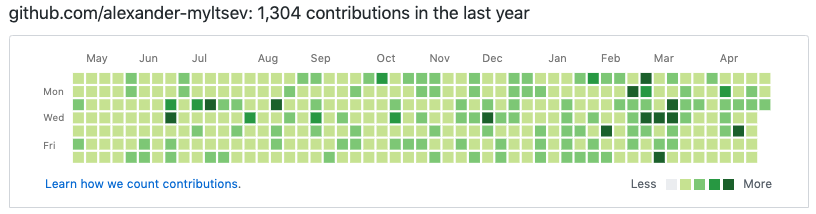
\includegraphics[width=\textwidth]{github-stats}}

\begin{samepage}
\begin{rSubsection}{\href{http://globalnames.org/}{Global Names Architecture
(http://globalnames.org)}}{June 2015 -- present}
{Full-stack Search Engine Developer}{\href{http://www.inhs.illinois.edu/}{Natural History Survey},
\href{http://illinois.edu/}{University of Illinois at Urbana-Champaign, USA}}
\item System of web-services which helps people to register, find, index, check and organize
biological scientific names and interconnect on-line information about species
\item I made significant contribution to dramatically speed up and improve quality of name parsing
(40x), name resolution and retrieval (10x), Biodiversity Heritage Library indexing (from 40 days to
1 day)
\item Co-designing production-ready search engine, applying algorithms and technologies in search,
machine learning, data mining and natural language processing
\item Paper: ``gnparser -- a powerful parser for scientific names based on parsing expression
grammars''
\item Using Scala Dev Stack, language parsing grammars, Python, Ruby, Angular/TypeScript, 
PostgreSQL/MySQL, Machine Learning and Natural Language Processing
\end{rSubsection}
\end{samepage}

\begin{samepage}
\begin{rSubsection}{\href{https://github.com/okama-io/yapo}
{Yet Another Assets Portfolio Optimization Library}}
{May 2017 -- present}{Co-author, core developer}
{\href{https://github.com/okama-io/yapo}{https://github.com/okama-io/yapo}}
\item delivers comprehensive functionality to the individual investor to compose and analyze
portfolios
\item implements facilities of modern portfolio theory by H.Markowitz
\item the crawler (MUTs, stocks, ETFs, currencies, countries inflation) and the library are
written in Python3
\end{rSubsection}
\end{samepage}

\begin{samepage}
\begin{rSubsection}
{\href{http://parboiled2.org}{parboiled2}}
{May 2013 -- present}{Co-author, core
developer}{\href{http://parboiled2.org}{http://parboiled2.org}}
\item Successfully completed Google Summer of Code '13 internship program. Contributed to a
real-world, long-term project: ``parboiled2 -- Macro-Based PEG Parser Generator for Scala''. Being
a part of a globally distributed team
\item Co-designed the overall architecture. Implemented most of the functionality till the present
moment
\item Paper ``parboiled2: macro-based parsing expression grammar generator for Scala programming
language''. Journal of Functional Programming (ISSN: 1469-7653, Online)
\textit{(\href{http://myltsev.com/papers/parboiled2.pdf}{draft})}
\item 606 stars at github. The project is in core of
\href{https://doc.akka.io/docs/akka-http/current/}{Lightbend Akka-HTTP}
\end{rSubsection}
\end{samepage}

\end{rSection}

%----------------------------------------------------------------------------------------
% HONORS & AWARDS SECTION
%----------------------------------------------------------------------------------------

\begin{rSubsectionSchools}{Honors \& Awards}
\item Oct 2015,  Machine Learning Hackathon (Microsoft) winner (MicroYandex team)
\item Sept 2013, R\&D Grant for [job]snipper, U.M.N.I.K.-MIPT (\$13000 USD)
\item Jun 2010, CUDA certified professional
\item Imagine Cup 2011 team, Russian finalists of Embedded Development
\item Best Report at VII All-Russian Conference ``Microsoft Technologies in Theory and Practice of
Programming'' in 2010
\item Imagine Cup 2010 team, 2nd place in a regional stage of Software Design Competition in Moscow
\& 4th place in Russian final of Embedded Development
\item Mozilla Labs Jetpack Contest 2009 winner: Mozilla Firefox Jetpack and NVIDIA CUDA
integration for data processing
\end{rSubsectionSchools}

%----------------------------------------------------------------------------------------
% WORK EXPERIENCE SECTION
%----------------------------------------------------------------------------------------

\pagebreak

\begin{rSection}{Experience}

\begin{samepage}
\begin{rSubsection}{\href{https://newprolab.com/en/bigdata/}{Digital October, New Professions Lab
(https://newprolab.com/en/bigdata/)}}{Mar -- Sept 2015}{BigData Course Tutor}{Moscow,
Russia}
\item Tutored 60+ students in Apache Spark, Python, HBase, Data Mining, Machine Learning
\item Improved course materials
\end{rSubsection}
\end{samepage}

%------------------------------------------------

\begin{rSubsection}{\href{https://www.vistohub.com/}{Collective Media
(https://vistohub.com/)}}{Nov 2013 -- May 2015}{External Scala Development Consultant}{New
York, USA / Moscow, Russia}
\item Helped to build high-loaded backend for ad-tagging server that serves 100K+ requests per
second
\item Introduced JMH benchmarking to the project. Optimized bunch of performance critical parts of
code
\item Advocated and contributed to open-sourced projects:
\href{https://github.com/kamon-io/Kamon}{kamon},
\href{https://github.com/sbt/sbt-aspectj}{sbt-aspectj},
\href{https://github.com/eigengo/monitor}{monitor},
\href{https://github.com/vspy/scala-mustache}{scala-mustache},
\href{https://github.com/Livestream/scredis}{scredis},
\href{https://github.com/etaty/rediscala}{rediscala},
\href{https://github.com/aphyr/riemann}{riemann}
\item Developed projects particularly for company needs:
\href{http://github.com/alexander-myltsev/RSlick}{RSlick} and
\href{http://github.com/alexander-myltsev/sbt-uglify}{sbt-uglify}
\item System performance analysis based on Hadoop logging processing
\item Contributed significantly to build system automation (SBT)
\item Distributed team work
\end{rSubsection}

%------------------------------------------------

\begin{rSubsection}{\href{http://nvidia.ru}{NVIDIA}}{Dec 2010 -- May 2012}{Contractor at CUDA
Certification and Tech Marketing Department}{Moscow, Russia}
\item The evangelist of CUDA technologies: certification program support, CUDA experts community
development, creating CUDA learning courses, tutorials, public talks
\item Invited speaker at Summer 2011, Winter 2011 and Spring 2012 Schools in GPU Computing and CUDA at Moscow State University
\item Co-author of the book ``Parallel computing on GPU Architecture and CUDA programming model'' and the corresponding online course for \href{http://hpc-education.ru}{hpc-education.ru}
\item Developed the cross-platform learning shell
\end{rSubsection}

\end{rSection}

%----------------------------------------------------------------------------------------
% TECHNICAL SKILLS SECTION
%----------------------------------------------------------------------------------------

\begin{samepage}

\begin{rSection}{Technical Skills}

\begin{tabular}{ @{} >{\itshape}l @{\hspace{6ex}} l }
Computer Languages & Scala, Java, Python, Scheme, Ruby, TypeScirpt, C\#, Haskell, F\#, C/C++, CUDA C/C++ \\
Dev Stack & SBT, Macros, Shapeless, Akka, spray.io, Play Framework, Anorm, Slick, Angular2 \\
Data tools & MySQL, PostgreSQL, Hadoop, Hive, Spark, Aerospike, Redis \\
Development tools & Microsoft Azure, Heroku, Docker, Ubuntu, bash, Nginx, Git, \LaTeX \\
\end{tabular}

\end{rSection}

\end{samepage}

%----------------------------------------------------------------------------------------
% TECH/INVITED TALKS SECTION
%----------------------------------------------------------------------------------------

\begin{rSubsectionSchools}{Tech/Invited Talks}
\item Biodiversity Information Standards Conference (TDWG) '17 in Canada. Talk: ``A path to
continuous reindexing of scientific names appearing in Biodiversity Heritage Library data''
\item Biodiversity Information Standards Conference (TDWG) '16 in Costa Rica. Talk: ``New
Scientific names finding, parsing and resolution tools from Global Names.''
\item
\href{https://www.youtube.com/watch?v=P4UusE7J2qc}
{ScalaDays.org 2014 conference} in Berlin, Germany. Talk: ``Meet parboiled2  -- a macro-based PEG
parser generator for Scala''
\item Speaker at Summer '11, Winter '11 and Spring '12 Schools in GPU Computing and CUDA at
Moscow State University
\end{rSubsectionSchools}

%----------------------------------------------------------------------------------------
% ADDITIONAL INFORMATION
%----------------------------------------------------------------------------------------

\begin{rSection}{Additional Information}

\begin{table}[h]
%\begin{tabularx}{ @{} >{\bfseries}l @{\hspace{6ex}} l }
\begin{tabularx}{\textwidth}{l X}
Languages & Russian (mother tongue), English (fluently reading technical documentation, verbal
proficiency adequate to pass a technical interview) \\
Personality & hard-working, responsible, research-driven, energetic, innovative, experienced to
work in globally distributed teams \\
Hobbies & Ashtanga Yoga, Total immersion swimming
\end{tabularx}
\end{table}

\end{rSection}

\pagebreak

\begin{rSection}{Competitive Programming}

\begin{itemize}
\item completed 1 semester course of competitive programming at
\href{https://vk.com/cs_hse_olymp}{Higher School of Economics} in 2018
\item regularly solve tasks at the \href{https://vk.com/35zvn}
{``3.5 Computer Tasks per Week'' project}
\item slow but positive progress trend at \href{https://codeforces.com/profile/solver}
{codeforces.com} from the beginning of 2019

\noindent\makebox[\textwidth]{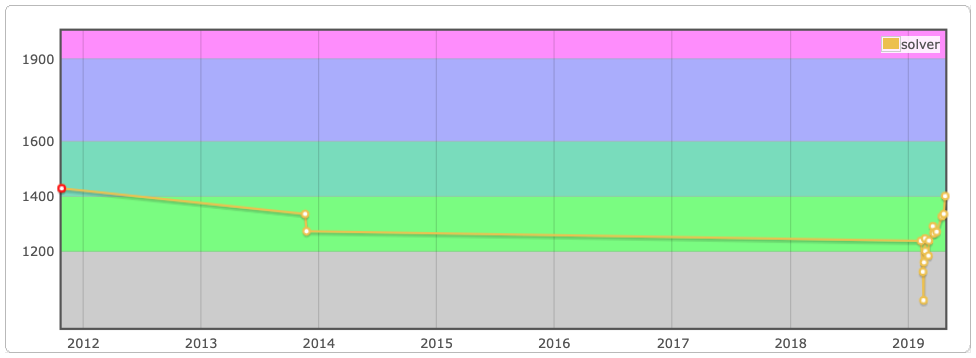
\includegraphics[width=\textwidth]{codeforces-progress}}
\end{itemize}

\end{rSection}

\end{document}
